\section{Data description}
One of the most straightforward way to deal with the limit amount of available data is to leverage as much related Medical Data as possible. We thus investigated several public available dataset for Lung CT scans in addition to the Covid-CT dataset.

\subsection{NSCLC Dataset}
NSCLC Dataset contains 402 Lung CT scans, of which 78 cases are anotated with left lung, right lung and pleural effusion area. A sample annotation is shown in figure \ref{fig:NSCLC_example}
\begin{figure}[h]
	\centering
	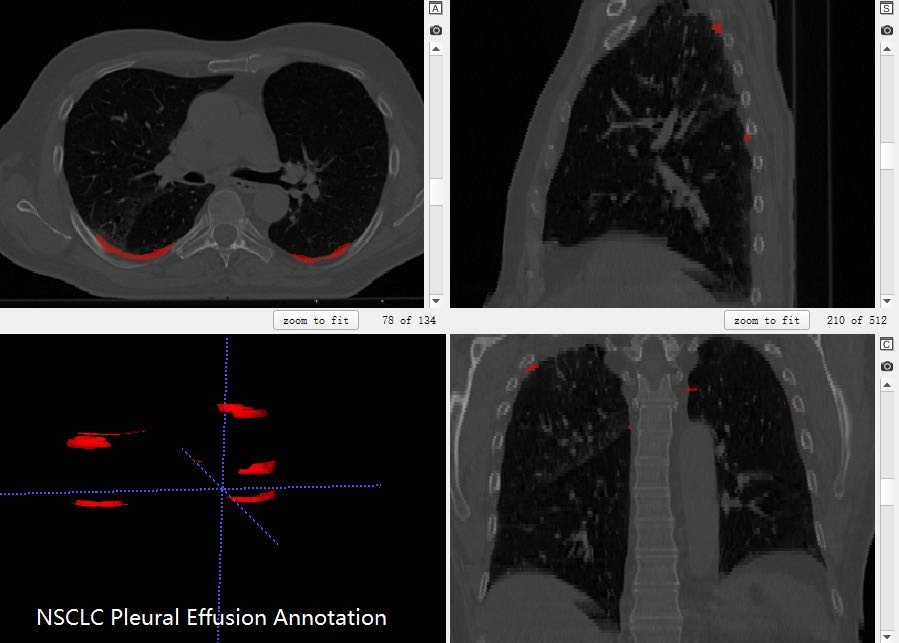
\includegraphics[width=0.6\textwidth]{img/Dataset/NSCLC}
	\caption{An example volume from NSCLC Dataset with its annotation}
	\label{fig:NSCLC_example}
\end{figure}

\subsection{MSD Lung Tumor}
MSD Lung Tumor contains 63 Lung CT scans, annotating the Lung Cancer area. An example shown in figure \ref{fig:MSD_example}
\begin{figure}[h]
	\centering
	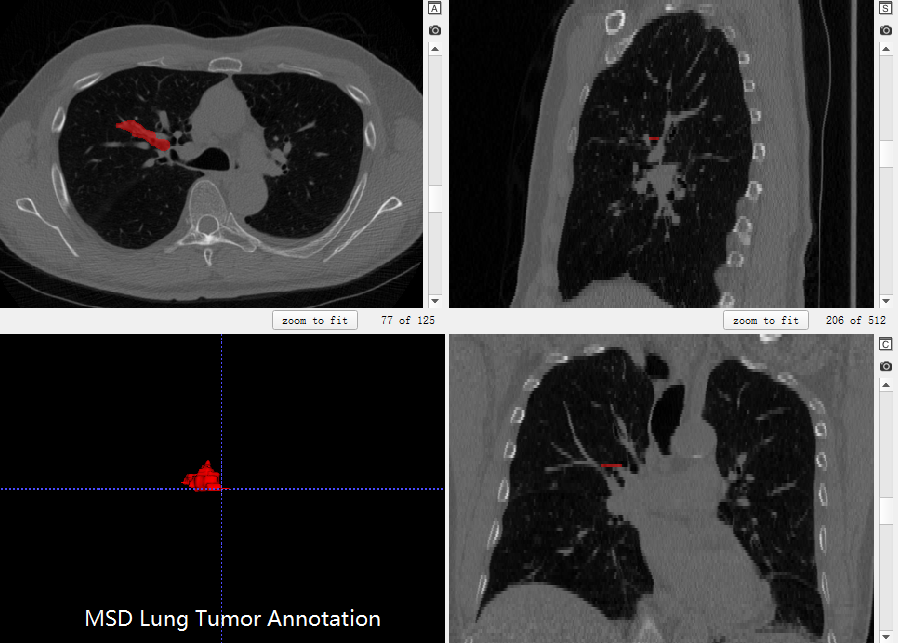
\includegraphics[width=0.6\textwidth]{img/Dataset/MSD}
	\caption{An example volume from MSD Dataset with its annotation}
	\label{fig:MSD_example}
\end{figure}

\subsection{MosMed Dataset}
MosMed Dataset Contains 50 Annotated thick-slice Covid CT scans, as well as around 300 unannotated Lung CTs. We'd like to report here that we used only 200 unannotated slices because downloading keep giving me error due to location restriction. An example shown in figure \ref{fig:MosMed_example}
\begin{figure}[h]
	\centering
	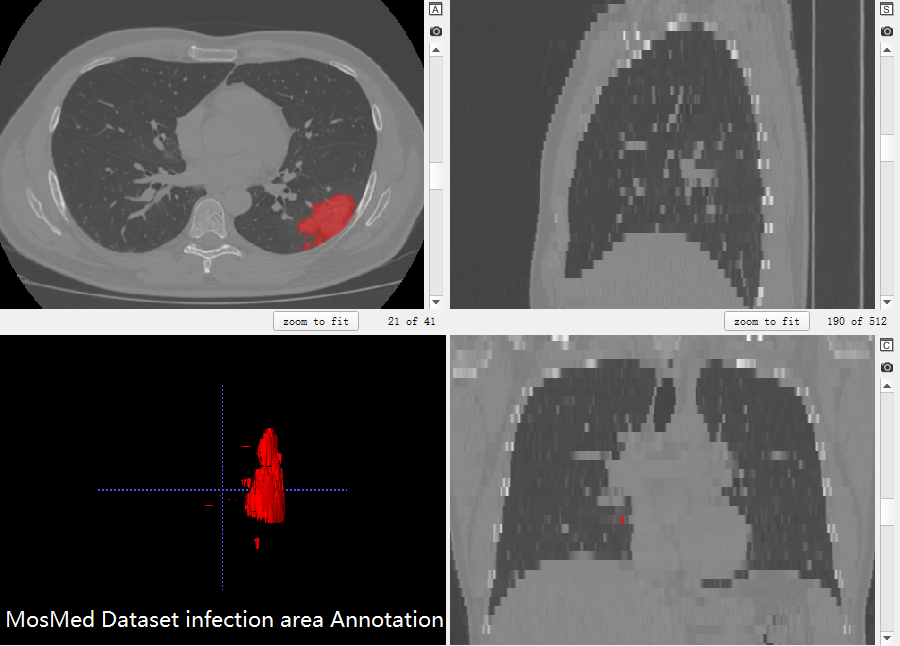
\includegraphics[width=0.6\textwidth]{img/Dataset/MosMed_example}
	\caption{An example volume from MosMed Dataset with its annotation}
	\label{fig:MosMed_example}
\end{figure}


\subsection{Covid Segmentation Benchmark}
Covid Segmentation Benchmard contains 20 CT scans from 2 radiometric centers, of which 10 volumes thin-slice CT volumes and 10 thick slice CT volumes.
\begin{figure}[h]
	\centering
	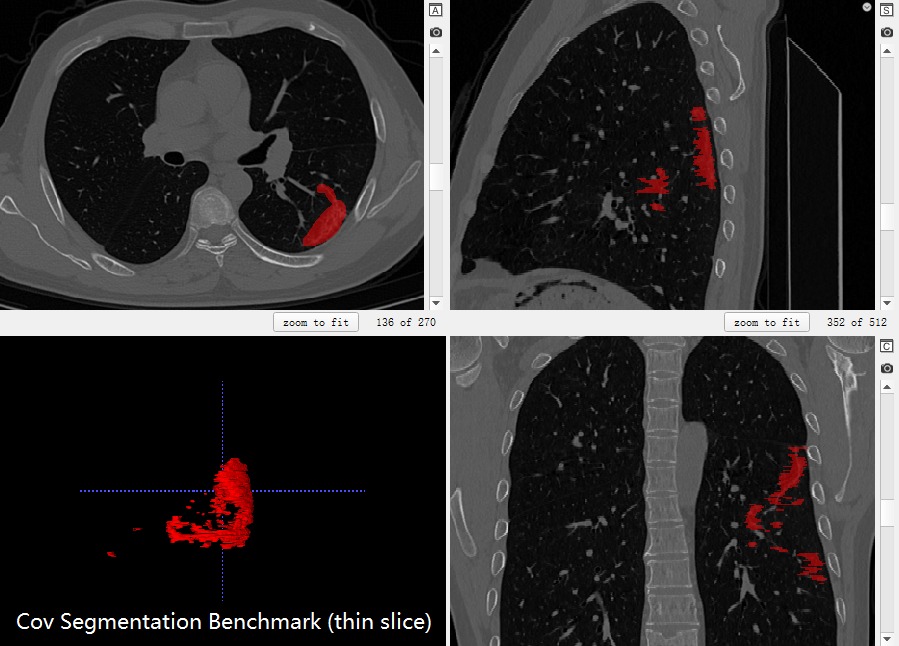
\includegraphics[width=0.6\textwidth]{img/Dataset/Cov_benchmark_thin}
	\caption{An example volume from Cov Segmentation Benchmark (thin slice) with its annotation}
	\label{fig:Covseg_thin}
\end{figure}
\begin{figure}[h]
	\centering
	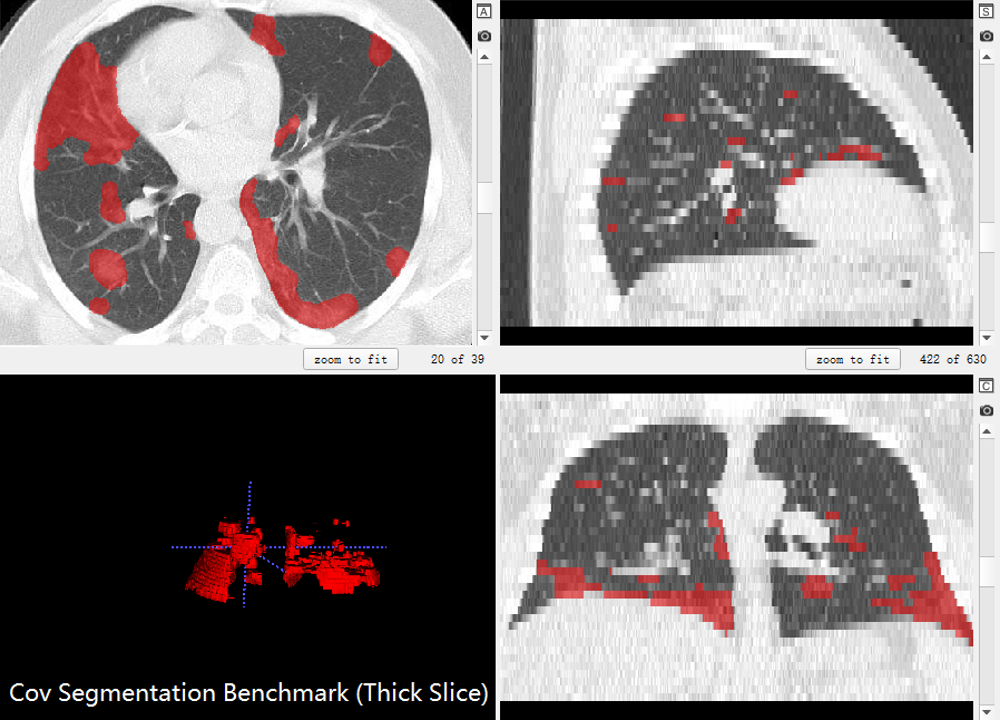
\includegraphics[width=0.6\textwidth]{img/Dataset/Cov_benchmark_thick}
	\caption{An example volume from Cov Segmentation Benchmark (thick slice) with its annotation}
	\label{fig:Covseg_thick}
\end{figure}


\section{Data preprocessing}
The dataset used in this paper was collected from multiple centers with different equipment setup. Structseg2019, NSCLC, MSD Lung Tumor set are thin slice CT scans. MosMed contained 50 thick slice scans and the Covid segmentation benchmark are multi-center dataset from different centers. We argue that deep learning algorithms, especially segmentation tasks are sensitive to this difference. To make most use of the data, we first extract the lungs from the CT volumes. Then a sequence of preprocessing was performed including resampling, histogram equalization, and mean variance normalization. Most implementation used SimpleITK dataset
\subsection{Data gathering and cleaning}

\subsection{Processing into functional features}
Lung CT scans images includes the lung tissue as well as bones and meshes that influence the preprocessing such as normalization as well as future segmentation. We intended to first segment the lung tissue out for better focus.\\
\textbf{Lung segmentation using watershed algorithm}\\

\textbf{Lung segmentation Using pre-trained Deep learning models}\\
Deep learning method provide finer results when facing severe pathology. Work in \cite{hofmanninger_automatic_2020} provided a promising result for Lung segmentation. In addition, they further improve their lung segmentation model with Covid-19 Lung data.\\

We leveraged their models provided in their github repository \footnote{https://github.com/JoHof/lungmask}. Original volumes from the Lung datasets went through the model, we threshold the lung out and set the uninterested area (background) as 0. Figure \ref{fig:filtered_Lung} showed and example lung volume before and after filtering the lung tissue.

\begin{figure}[h]
\centering
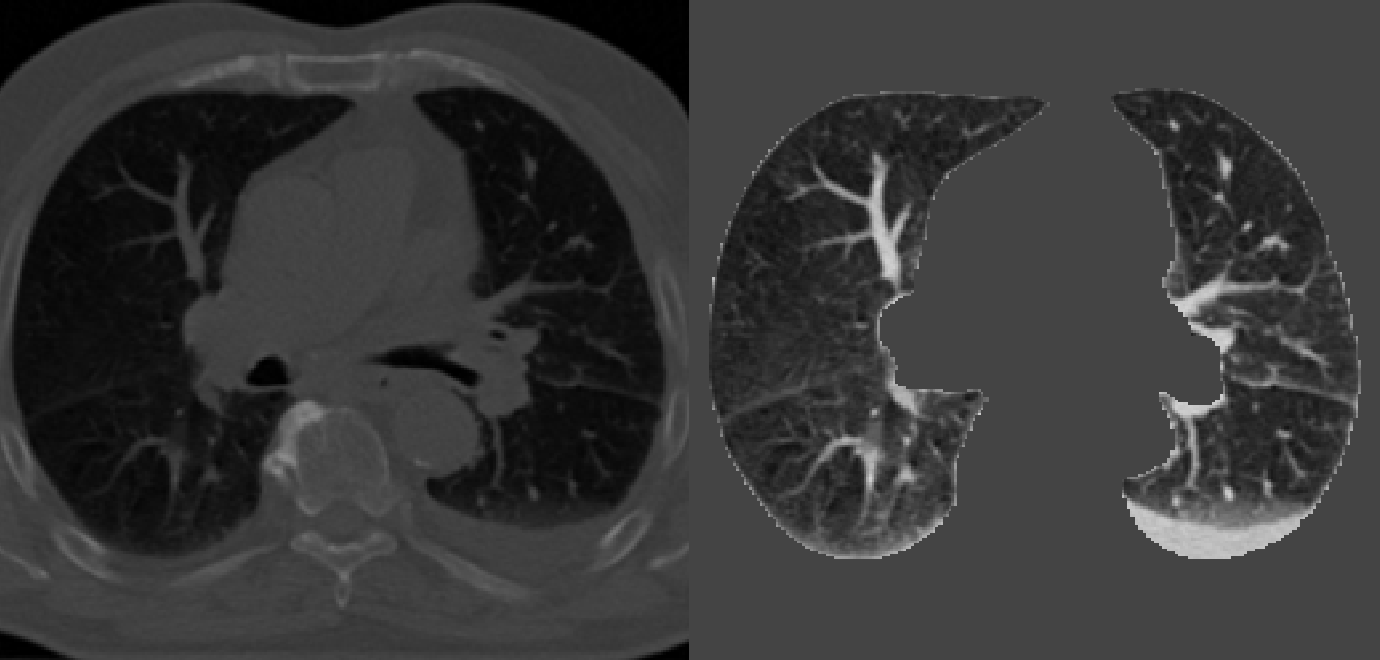
\includegraphics[width=0.5\textwidth]{/Users/tianyangsun/Desktop/Project/MSc-report/img/filtered_lung/nsclc_filteredlung_axial.png}
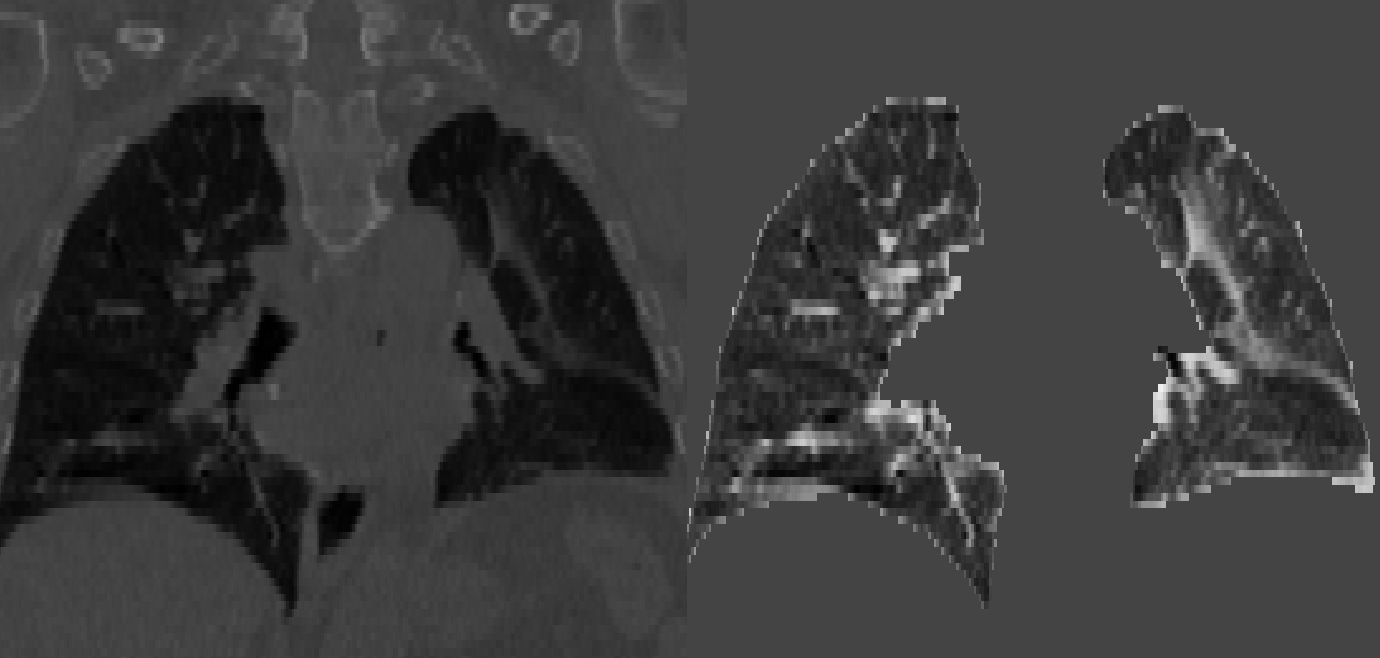
\includegraphics[width=0.5\textwidth]{img/filtered_lung/nsclc_filtered_coronal.png}
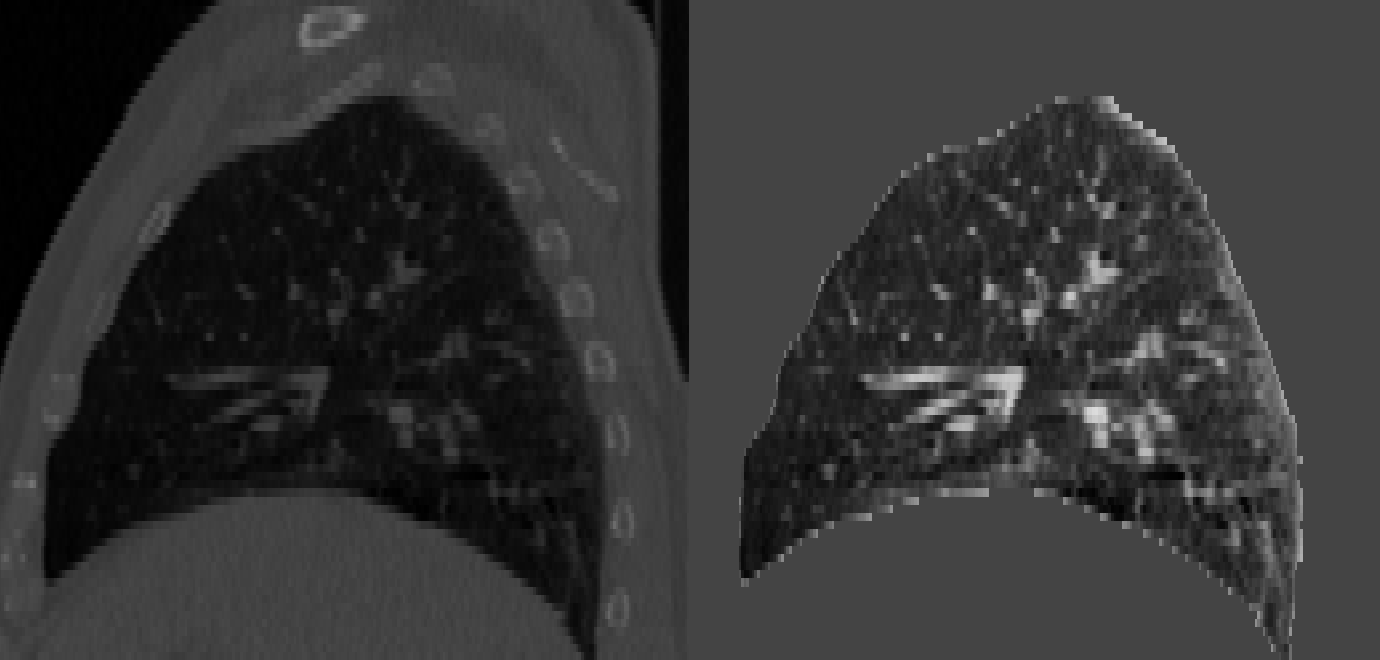
\includegraphics[width=0.5\textwidth]{/Users/tianyangsun/Desktop/Project/MSc-report/img/filtered_lung/nsclc_filteredlung_Saggital.png}
\caption{An example from NSCLC Pleural Effusion dataset showing the volumes before and after lung filtering. (Top: Axial view, Middle: Coronal view, Bottom: Saggital View)}
\label{fig:filtered_Lung}
\end{figure}

\subsection{Resampling}
\begin{figure}[h]
	\centering
	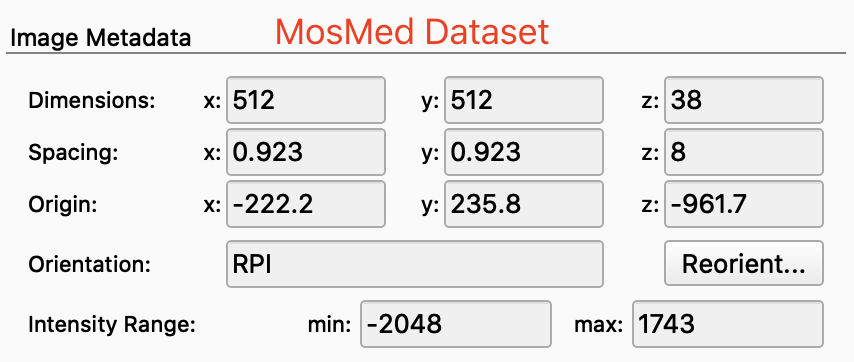
\includegraphics[width=0.5\textwidth]{/Users/tianyangsun/Desktop/Project/MSc-report/img/spacing_diverse/Mosmed_dataset.png}
	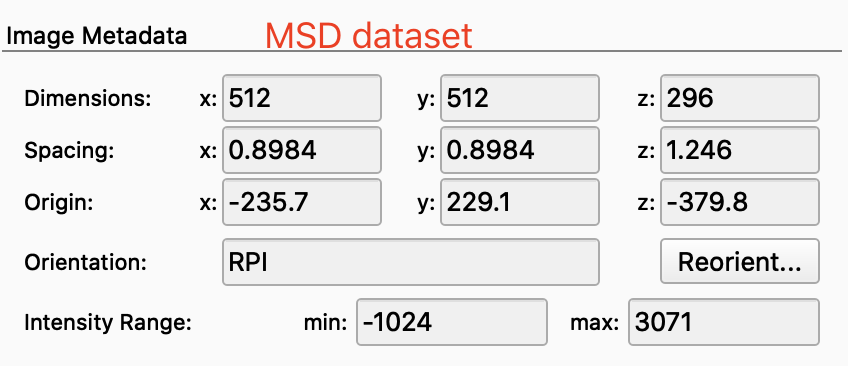
\includegraphics[width=0.5\textwidth]{/Users/tianyangsun/Desktop/Project/MSc-report/img/spacing_diverse/MSD_metadata.png}
	\caption{An example of different spacing information from MosMed and MSD dataset}
	\label{fig:Spacediverse}
\end{figure}
Figure \ref{fig:Spacediverse} showed the diveristy in spacing from different datsets. To deal with the different spacing for multi-domain data, we resampled the data to spacing (1, 1) in the Axial view and remain not changed in the Z axis.

\subsection{Mean Variance Normalization}
We performed Mean Variance Normalization (Z score normalization) for the lung tissue voxels by subtracting each volume with its mean and divided by its standard deviation. So that the data has zero mean and standard deviation of 1. 
$$z=\frac{x-\mu}{\sigma}$$ of which $\mu$ is the mean and $\sigma$ is the variance. Figure \ref{fig:normalization} showed the intensity range before and after normalization

\begin{figure}[h]
	\centering
	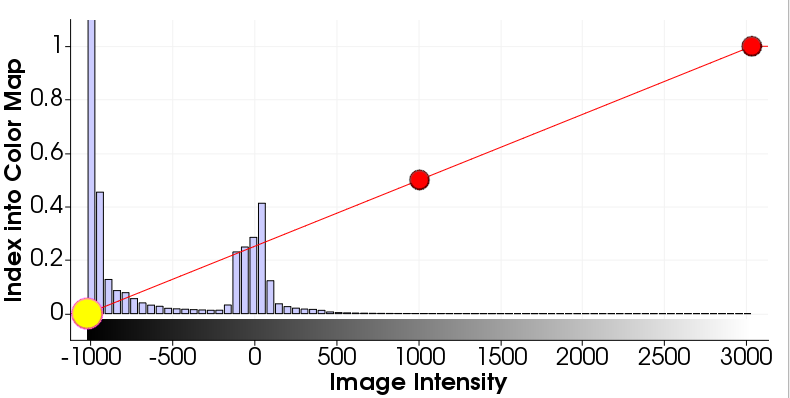
\includegraphics[width=0.5\textwidth]{/Users/tianyangsun/Desktop/Project/MSc-report/img/normalization/intensity_before.png}
	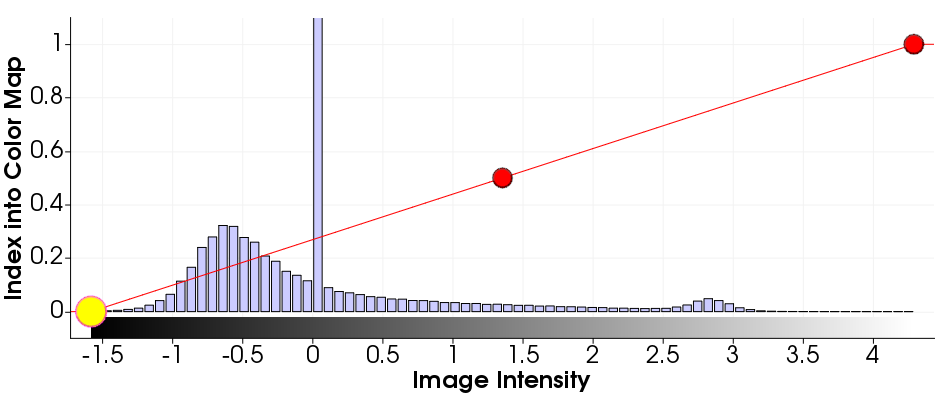
\includegraphics[width=0.5\textwidth]{/Users/tianyangsun/Desktop/Project/MSc-report/img/normalization/intensity_after.png}
	\caption{An example showing the intensity range before and after normalization (Top: before normalization; Bottom: after normalization)}
	\label{fig:normalization}
\end{figure}

\newpage
\section{Data Augmentation}
% TODO: add examples showing the transformation in augmentation
For data augmentation, we investigated some of the augmentation techniques in medical imaging domain, each of the augmentation techniques was carefully chosen matching real medical situation.\\

\textbf{Rotation:} We performed a small random rotation between [-3, 3] degree considering the pose variation when lying down on the scanner.\\
\begin{figure}[h]
	\centering
	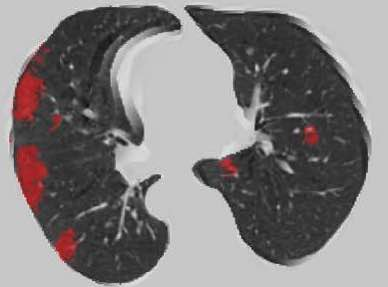
\includegraphics[width=0.4\textwidth]{img/augment/rotation}
	\caption{An example of rotation using MosMed Dataset}
\end{figure}

\textbf{Elastic Transformation:} We performed a small elastic transformation considering lying down and holding breath when scanning Lung CT might brings shape change to the lungs tissue.\\
\begin{figure}[h]
	\centering
	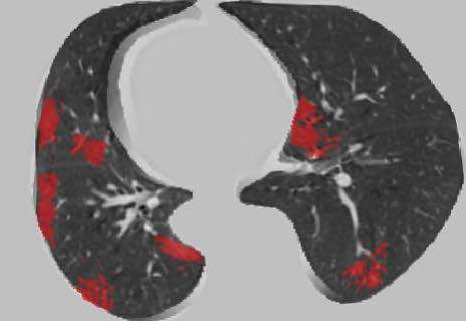
\includegraphics[width=0.4\textwidth]{img/augment/elastic_transformation}
	\caption{An example of elastic transformation using MosMed Dataset}
\end{figure}

\textbf{Random Gamma and Gaussian Noise:} We performed a random gamma correction to simulate the variation generate due to different equipment. We also added a random gaussian noise for a more robust training.

\begin{figure}[h]
	\centering
	\includegraphics[width=0.4\textwidth]{img/augment/add_noise}
	\caption{An example of random Gamma and Gaussian Noise using MosMed Dataset}
\end{figure}


